% -*-LaTeX-*-

% $Log: review.tex,v $
% Revision 1.3  2007/03/20 22:45:23  stiber
% Modified for stand-alone textbook use.
%
% Revision 1.2  2004/03/29 19:55:49  stiber
% Updated for Spring 2004 and new textbook (DSP First).
%
% Revision 1.1  2004/02/19 00:28:20  stiber
% Initial revision
%

\chapter{Review and Conclusions}
\label{ch:review}

This chapter brings our journey to a close. In an in-person course, we
would spend some time in lecture reviewing the material covered; this
of course is redundant here, as you have access to all that material
verbatim on-line. You also have access to the instructor for any
questions you might have. Instead, what we will do is examine a generic
multimedia system that includes all the course material, then describe
an example media system and relate its design to what we've learned in
this course. The system in question is the compact disc player, which
should be familiar to everyone and which is simple enough conceptually
that we can actually describe it in this limited space (at least, in
simplified form).

\section{A Generic Digital Multimedia System}

\begin{figure}
\centerline{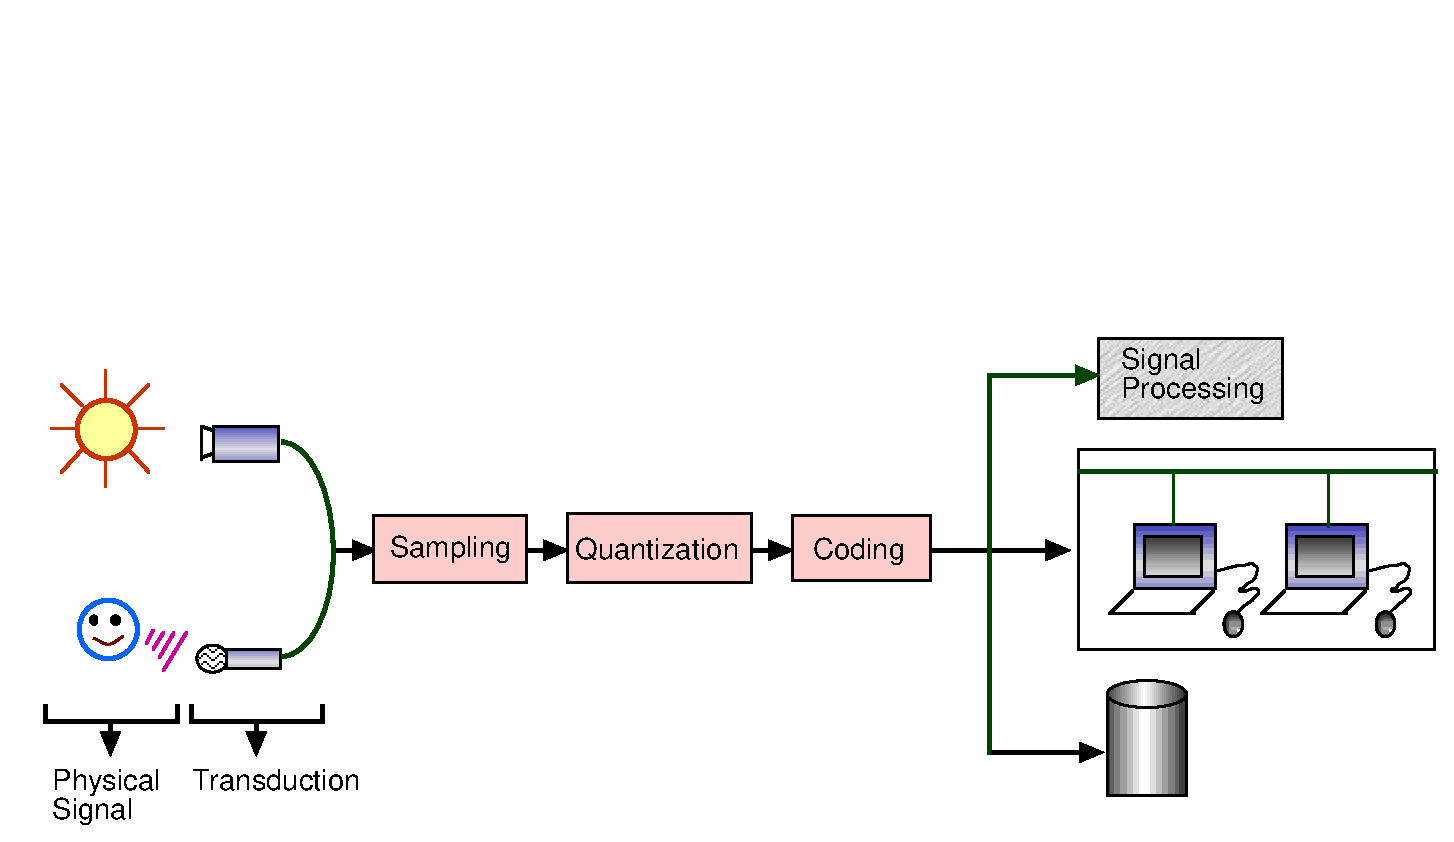
\includegraphics[height=4in,angle=-90]{ch-rev/fig10-1}}
\caption{Block diagram of a generic multimedia system.\label{fg:genmmsys}}
\end{figure}

Figure~\ref{fg:genmmsys} presents a simplified generic multimedia
system which highlights the concepts covered in this course. All
multimedia begins with physical signals --- light, sound,
etc. (Actually, that last statement isn't 100\% true, as there
\emph{is} such a thing as computer-generated multimedia: computer
music, computer graphics, etc.) These signals must be converted into
analog electrical signals so they can be captured by computer (or, for
that matter, so they could be recorded on analog media).  Digitization
involves converting the continuous-time analog signal to a
discrete-time signal via sampling. The sampled signal is then
quantized to a fixed number of bits of resolution per sample.  The
result is a \emph{digital signal}. This raw signal is typically
encoded for compression purposes and/or to add information to the data
stream (for example, error correction codes).

At this point, the encoded signal can be treated like any other
digital information manipulated by computer. It can be stored in
files, transmitted over networks, processed to improve or alter it,
and/or presented to human beings on a desktop computer (or, these
days, a consumer device like an HDTV set).

\section{Compact Discs}

One example digital multimedia system is the compact disc, or more
precisely, since I'm referring to music CDs, compact disc digital
audio (CD-DA). The standards associated with CDs (the \textit{Red
Book}, defined by Philips and Sony in 1980 so that discs would be
\index{CD-DA}
\index{red book}
interchangeable among different manufacturers' hardware, and IEC
Publication 60908) cover the disc itself and the optomechanical drives
that spin it and read from it.

Information is recorded onto a CD in the pattern of pits and bumps (or
\emph{lands}) of a metal layer sandwiched between two covering plastic
\index{lands}
layers.  These pits and lands are arranged in a spiral pattern, like a
vinyl LP. There are two differences between the CD layout and the LP:
data is recorded from the innermost part of the surface outward and
the disc's rotation speed changes as the read laser moves. The change
in rotation speed is necessary because a CD is a constant linear
velocity (CLV) device: rotation speed is set so that the data moves
past the read laser at the same rate everywhere on the disc. Near the
center, the disc rotates at 500 rpm; this slows to 200 rpm at the
outer edge. The rotation rate is automatically regulated by the drive
mechanism to maintain a constant data rate of 4.3218 Mbps.

Data is read from the disc by a laser/detector pair. The laser
illuminates a spot on the underside of the disc and the metal layer
reflects this back to the detector. About 90\% of the laser light is
reflected by a land; pits, on the other hand, reflect only about 25\%
of incident light. This difference is easily detectable, and thus the
\emph{encoded} data can be read.

\subsection{Data Encoding}

Data is encoded on a CD so as to both minimize the effect of and
correct for errors. This is especially important for a device that has
an exposed surface and is intended to by used by ordinary consumers.
Even without these considerations, error correction would be important
in a device where a speck of dust could wipe out 50 bits on each of
ten spirals. The CD standard uses a number of techniques to encode
data so that commonly-expected errors can be detected and corrected.

\index{error correction!in compact discs|(}
The first thing we note about error detection and correction is that
it will require extra information to be sent. In effect, redundancy is
introduced into the data stream in a manner such that errors are
unlikely to destroy both the ``original'' and the ``copy''. (In
reality, of course, the scheme is more sophisticated than just
recording copies of the data.) From this, you should conclude that the
data stream is not maximally compressed; in fact, CD audio is recorded
uncompressed as 16 bits/sample, linearly encoded (i.e., no
companding). Error detection and correction schemes involve adding
bits (an \emph{error correction code}) to each byte (or larger group)
of data.

\subsubsection{Error ``Clumps''}

If you consider the error generated by a scratch, dust, etc., it seems
that this will obliterate a large number of consecutive data bits: a
``clump'' of data bits.  This would seem guaranteed to eliminate not
only the original data, but also the associated error correction
codes.

To reduce the probability of errors in long, contiguous stretches of
data, a simple scheme is to not record long, contiguous stretches of
data.  After all, if you don't record them, then you can't get those
kinds of errors, right? This is accomplished by \emph{interleaving}:
data is shuffled before being recorded, so that errors in contiguous
sections on the disc will correspond to isolated errors in the
data. To demonstrate this effect, let's say that we record the numbers
one through ten in shuffled order: 1, 10, 5, 2, 9, 6, 3, 8, 4,
7. Suppose a clump of errors occurs in the second, third, and fourth
numbers, rendering them unreadable. The result is:
\begin{displaymath}
\begin{array}{rcl}
\begin{array}{|c|c|c|c|c|c|c|c|c|c|}\hline
1 & \hphantom{10}  & \hphantom{5} & \hphantom{2} & 9 & 6 & 3 & 8 & 4 & 7 \\ \hline
\end{array} &
\Longrightarrow &
\begin{array}{|c|c|c|c|c|c|c|c|c|c|}\hline
1 & \hphantom{2} & 3 & 4 & \hphantom{5}  & 6 & 7 & 8 & 9 & \hphantom{10}\\ \hline
\end{array}
\end{array}
\end{displaymath}
Errors in three consecutive words on disc are widely separated in the
de-interleaved data stream. An appropriate interleaving stream,
shuffling data over a wide area, can cause clumps of errors to become
widely distributed, and thus more likely to be correctable using the
surrounding intact information. In the CD standard, the interleaving
and error correction scheme is called \emph{Cross Interleave
Reed-Solomon Code}, or CIRC.
\index{Reed-Solomon code (CIRC)}

\subsubsection{``Faking It''}

Sometimes, an error will occur which is too massive for the error
correction scheme. To prevent unpleasant listener experiences, CD
players use varying two schemes to mask such errors: interpolation and
muting.

In \emph{interpolation}, the ``good'' waveform before and after the
\index{interpolation}
error is used to fill in the bad section with an approximation of what
it might have been. A simple approach would be to just repeat the last
good data value to fill in the gap; a better method would be to
linearly interpolate between the two data values on either side of the
gap. Interpolation schemes also can be used which ``blend'' the
interpolated values into the gap ends more smoothly than a straight
line does.

At some point, the gap becomes too big for interpolation. The
workaround employed is \emph{muting}: the volume of the music is
\index{muting}
smoothly reduced before the gap and increased back up afterwards.
This avoids unpleasant effects like lound pops and clicks.
Additionally, by fading out and back in smoothly, the problem is less
noticable (sometimes even unnoticable).

\subsubsection{Error Performance}

CDs are not error-free devices. In fact, the typical number of errors
in the raw data from a CD is one in 100,000 to 1,000,000 bits. I've
already mentioned that the data rate from the CD is over 4 million
bits per second, so we should expect many errors per second. CIRC
error correction can repair most of these errors.  Depending on the
particular player's implementation (and this is never listed in the
specs for an audio CD player), CIRC can deal with error clumps of up
to 4000 bad bits.  After CIRC, the error rate can be as low as one in
10--100 billion bits (if the player uses a good implementation; there
is no requirement that all of the error correction capability in CIRC
be used by the player to correct errors). In practice, a CD in
reasonably good shape might have one uncorrected error, which would
have to be dealt with by interpolation or muting.
\index{error correction!in compact discs|)}

\subsubsection{The Data Encoding Process}

CD-DA data is considered to be in two stereo channels sampled at
44.1kHz at 16 bits/sample. The samples from each channel are arranged
in alternating order (left 16 bits, right 16 bits, etc.) to yield
32-bit sampling periods. Six of these sampling periods will be encoded
as one \emph{frame} of data.

The next step towards assembling the frame is computing error
correction coding using CIRC. The data is treated as a sequence of
8-bit symbols for this process (so each sample corresponds to two
symbols). Four bytes of CIRC parity are added after the first 12 bytes
of data and four are added after the second 12 bytes. So, the original
24 bytes of data has now become 32 bytes.

Each frame then has a \emph{subcode} byte prepended to it.  The
subcodes in each frame contain information about the number of tracks
on the disc, their start and end times, etc. Each bit of a subcode
byte has a separate meaning, and a player collects these bits from 98
consecutive frames to produce eight 98-bit words with this
information. This might not seem like much information, but on a full
CD it would correspond to 32MB!

\begin{table}
\caption{Part of the eight-to-fourteen modulation lookup
table.\label{tb:efm}}
\begin{center}
\begin{tabular}{cc}
\textbf{Data Symbol (8 bits)} & \textbf{CD Word (14 bits)}\\
00000000 & 01001000100000 \\
00000001 & 10000100000000 \\
00000010 & 10010000100000 \\
00000011 & 10001000100000 \\
00000100 & 01000100000000 \\
00000101 & 00000100010000 \\
00000110 & 00010000100000 \\
00000111 & 00100100000000
\end{tabular}
\end{center}
\end{table}

At this point, the data is ready to be converted to the form which
will be recorded on the disc. Because of fabrication imprecision and
other manufacturing considerations, CDs do \emph{not} use pits to
encode zeros and lands to encode ones (or vice versa). Instead, ones
\index{lands}
are encoded as a pit-land or land-pit transitions, while zeros produce
no transitions. So, the rate of transitions (the length of pits or
lands) depends on how often ones are encountered in the data stream
(or, equivalently, the length of runs of zeros in the data). It is
desirable to control this so that all pits fall within some range of
minimum to maximum length. To accomplish this, each 8-bit symbol is
converted to a 14-bit pattern using \emph{eight-to-fourteen
modulation} (EFM). This is done via a look-up table, a portion of
\index{eight-to-fourteen modulation (EFM)}
which is presented in table~\ref{tb:efm}. The bit patterns in each
14-bit word are selected to generate a particular rate of occurrence
of ones (and, as a result, set the typical land and pit lengths). In
particular, only those words with more than two but less than ten
zeros in a row are chosen.  Additionally, since only 256 of the
possible 16K 14-bit words are used, those words are less similar than
the original symbols, which yields some additional error correction
capability. For example, with 256 8-bit symbols, if we flip a bit in
one symbol, we get another one. With only 256 out of 16K 14-bit words
used, flipping one bit is unlikely to produce another valid word
(about a 1.5\% chance).

There is still a need to control the transition between these 14-bit
words and to fix the ratio of high to low bits. So, between each pair
of words, three \emph{merging bits} are inserted. Two of these are
used to ensure that, even if the first 14-bit word ends with a one and
the next starts with a one, there won't be two ones in a row. The
third bit is chosen to be either a zero or a one to keep the overall
ratio at 8:17.

Frames of data are now indicated by adding a 24-bit synchronization
pattern before each: 100000000001000000000010 plus three merging
bits.  This is a set of three ones separated by tens zeros between
each pair, and won't appear anywhere else in the data. Besides marking
the start of a frame, this is used by the player as a clock to
regulate rotation speed. The resultant frame contains 588 bits: 24
synchronization pattern bits, 336 data bits (in 24 14-bit words), 112
error correction bits (in 8 14-bit words), 14 subcode bits, and 102
merging bits (in 34 groups of three bits each).

The data is ready for recording at this point. Pit edges encode ones;
while the extent of pits or lands correspond to zeros. The data stream
has been encoded so that all pits and lands are between 3 and 11 bits
long (in other words, there are between 3 and 11 zeros in a row
anywhere in the data).

The result of all this is that only about 32\% of the data on a disk
is the actual audio information; the rest is overhead of EFM, merging
bits, CIRC, synchronization, and subcodes.

\subsection{CD System Signal Processing}

\begin{figure}
\centerline{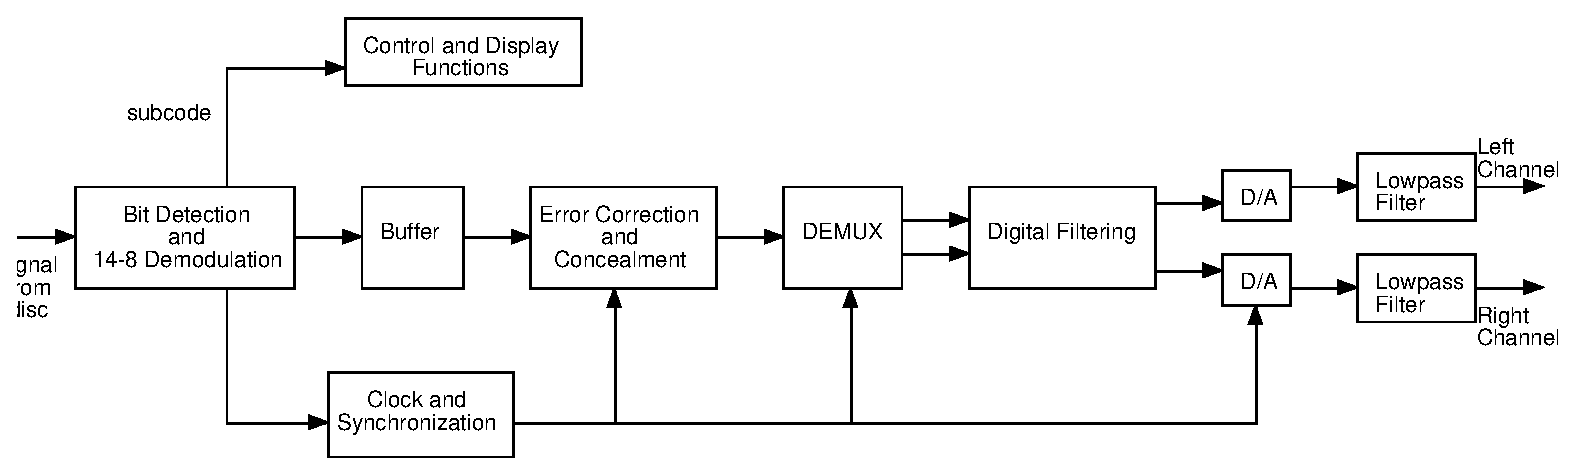
\includegraphics[width=\textwidth]{ch-rev/fig10-2}}
\caption{Simplified block diagram of a CD player.\label{fg:cd-player}}
\end{figure}

A CD player converts the information encoded on the disc into analog
audio. Figure~\ref{fg:cd-player} is a simplified block diagram of a CD
player. Processing begins with detection of the pit/land transitions
from the disc (which includes a control system that maintains the
appropriate spindle rotation speed, moves the laser along the track of
the pits, and keeps the laser focused on the metalized layer within
the disc). This raw data then has the merging bits removed, and is
converted from 14-bit words to 8-bit symbols. The subcode symbols are
sent to a parallel pathway to support the player's user interface.

The data symbols are stored in a queue that leads to further
processing.  The first step of this is error detection, correction (if
possible), and concealment (if uncorrectable). The two channels (left
and right) are then separated (\emph{demultiplexed}; ``DEMUX'' in the
\index{demultiplex (DEMUX)}
figure). 

Next, digital filtering involves an \emph{oversampling}
transformation, in which additional samples are interpolated between
the original ones, and a low-pass filter. Oversampling results in one,
three, seven, or more interpolated values being inserted between each
pair of input samples. The result is a data stream which ``simulates''
one sampled at twice, four times, eight times, etc. the original rate
of 44.1kHz. ``Simulates'' is used here because any aliasing has already
occurred when the music was originally digitized (before it was
recorded to disc). The purpose of oversampling here is to produce a
digital signal with no information beyond 22.05kHz (the original Nyquist
limit imposed by sampling) but with a Nyquist limit of 44.1, 88.2,
176.4kHz or more. This allows the use of analog lowpass filters on the
output with frequency responses which drop off relatively gently
beyond 22.05kHz that still do not pass any undesirable high-frequency
artifacts.  Question: what's wrong with low-pass filters with abrupt
cutoffs (sometimes called \emph{brick wall} filters) (answer
in~\ref{sc:ch10ex}
\#\ref{it:ch10ex1})?

\begin{figure}
\centerline{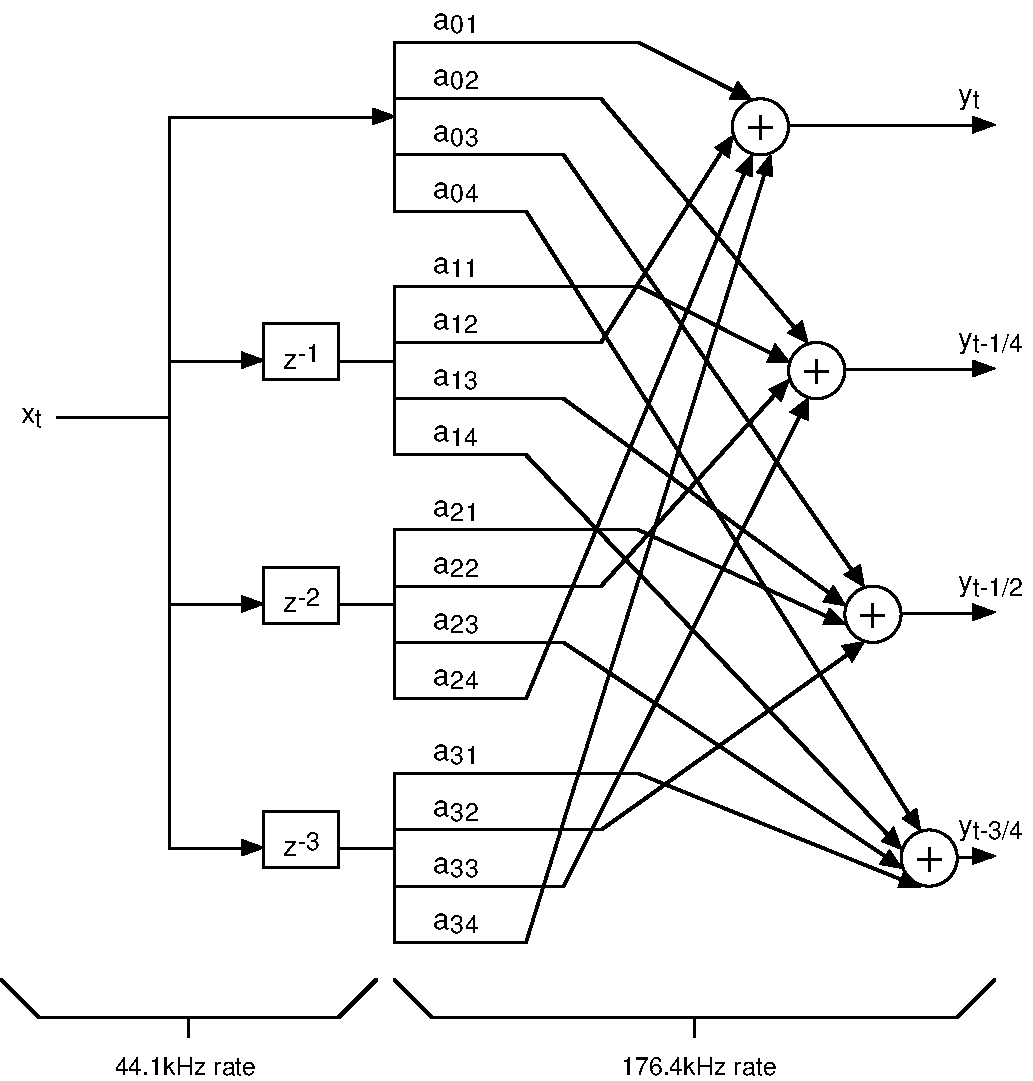
\includegraphics[height=5in]{ch-rev/fig10-3}}
\caption{Simplified oversampling filter.\label{fg:oversampling}}
\end{figure}

Figure~\ref{fg:oversampling} presents a simplified four-times
oversampling filter. In this simplified version, an input sample plus
three delayed versions are summed together to produce four output
samples. The coefficients are chosen so that a low pass filter with
cutoff at the input's Nyquist limit (22.05kHz) is implemented for each
output. The input samples enter at 44.1kHz (and thus the delays are
multiples of the sample period,
$T_s=1/44,100=22.7\mu\mathrm{s}$). During each input sample period,
each of the $xt$ values is multiplied by four different coefficients
and those products summed to produce four $y_t$, at a rate of
176.4kHz. This is then converted to analog by digital to analog
converters (D/A or DAC), and then low pass filtered before being sent
to the preamplifier, power amplifier, speakers, and your ears.

\section{Conclusion}

While it may have at times seemed a long and arduous journey,
hopefully, looking back, you have a sense of satisfaction in the scope
of understanding you've gained in this important subject.  Digital
multimedia is a big subject, and no single course can cover
everything. However, please consider the CD overview that you've just
gone through, the background required to understand it, and how
incomprehensible even the basics would likely have been to you before
you took this course.  I'd like you to use this experience to make you
confident that you could work in a team building multimedia devices,
be they digital audio, video, or telecommunications (wired or
wireless). The authors hope that this has served to whet your appetite for
more, and that you'll look for the implications for multimedia when
learning about databases, or hardware, or networking, or almost any
area of computing.

\section{Further Reading}

\begin{itemize}
\item Pohlman, Ken, \textit{The Compact Disc Handbook}, A-R Editions,
  1992.
\end{itemize}
